\chapter{Introduction}
This chapter presents the project’s background, core objectives, proposed methodology,
and expected outcomes, establishing the foundation for a real-time machine learning anxiety detection engine coupled with a high-fidelity interactive UI/UX adaptive intervention design framework.


\section{Project Overview}

The project outlines the design and evaluation of a two-stage developer well-being framework: a real-time machine learning anxiety detection backend coupled with a high-fidelity interactive UI/UX adaptive intervention system, conceptualized as a non-intrusive plugin environment for the CodeBlocks IDE. The background infrastructure passively collects behavioral indicators of coding activity, including keystroke velocity metrics, compile errors, idle time plateaus, and the structural frequency of undo/redo actions \cite{zhang2023keystroke, epp2015emotion}. A supervised machine learning classification algorithm is then applied to infer the programmer’s distinct anxiety level based on these extracted behavioral features \cite{acm345697, anxietyPrediction2023}. Depending on the detected affective state, the system theoretically maps out a context-aware intervention layer. This architecture introduces adaptive feedback mechanisms, reassurance prompts, and workflow pacing layouts designed to actively lower anxiety metrics, mitigate workflow friction, and elevate the overall psychological well-being of programmers \cite{selfreg2023, arean2025jitai}.

\section{Motivation}

As a highly cognitive and logic-heavy mental process, programming comes with inevitable affective side effects such as anxiety, stress, and structural frustration, particularly among novices and students operating under strict time constraints \cite{acm4897123, springer2020}. Being preoccupied with compiling blockages or errors can severely impair human problem-solving capacity, reduce debugging efficiency, and negatively impact overall learning performance \cite{stemedu2025}. Despite being designed to facilitate syntax accuracy and structural productivity, current IDE environments are completely unable to address the emotional states of users, including stress or panic loops, which significantly affect real-world programming performance \cite{mdpi5739}. It is becoming more necessary than ever to design lightweight, non-invasive, and IDE-based solutions capable of detecting behavioral stressors in real time \cite{realtimeStress2012}. These tools are expected to benefit both computer science students and engineering professionals by fostering better emotional self-regulation, preserving task motivation, and refining the general coding experience.


\section{Objectives}
The broad objective of this project is to develop an intelligent, non-intrusive, real-time anxiety detection system using an empirically validated machine learning processing backend, mapped directly to a comprehensive, multi-tiered interactive UI/UX adaptive intervention design configured for the CodeBlocks environment \cite{mdpi389}.

The specific objectives of the project are:
\begin{itemize}
    \item To design a non-intrusive software telemetry data collector capable of operating quietly in the background of a developer's coding environment without causing system latency or distracting the user.
    
    \item To monitor and evaluate passive behavioral coding features, specifically tracking typing speed fluctuations, latency variance, background window context-switching, and backspace usage to isolate reliable patterns of developer stress \cite{bunia2024keystroke}.
    
    \item To train, validate, and deploy a supervised machine learning model capable of predicting distinct anxiety risk levels through the systematic analysis of real-time coding behavior \cite{anxietyPrediction2023}.
    
    \item To architect a theoretical, context-dependent intervention engine mapped entirely via high-fidelity interactive prototyping, defining precise user-control nodes like soothing toast alerts, break recommendations, and guided relaxation exercises \cite{arean2025jitai}.
    
    \item To minimize interface friction with the user's primary programming task, ensuring that developer productivity and affective well-being stay the absolute priority of the layout \cite{codereview2024}.
    
    \item To compare the performance of the system's tracking features with both subjective metrics (self-reports about anxiety levels) and objective measurements (number of syntax errors, focus switches, and typing velocity variations).
    
    \item To guarantee high ethical standards through the use of transparent data collection boundaries, explicit user authorization protocols, and localized anonymous data processing to protect sensitive user telemetry.
\end{itemize}

\section{Methodology}
The project workflow follows an engineering design process structured across two parallel tracks: backend machine learning development and human-centered interaction design. The complete pipeline is divided into distinct phases: System Development, Data Collection, Feature Engineering, Model Training, and High-Fidelity UI/UX Prototyping. As shown in Figure~\ref{fig:methodology}, the System Development Phase forms the technical groundwork for the rest of the operational phases. Next comes Data Collection and Feature Engineering followed by Model Training and Interactive Frontend Interface Mapping, together making up the end-to-end evaluation framework.

\begin{figure}[htbp]
    \centering
    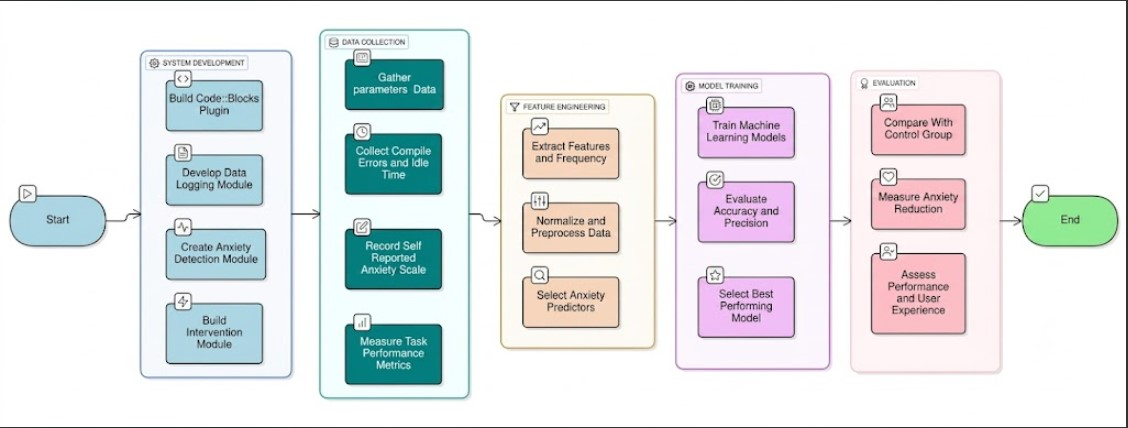
\includegraphics[width=\textwidth]{Methodology.jpg}
    \caption{Methodology and multi-stage system workflow for the anxiety detection system and prototype framework.}
    \label{fig:methodology}
\end{figure}

\subsubsection{1.4.1 System Development}
In this initial stage, the emphasis is placed on the basic engineering and architecture of the application tool infrastructure. This stage includes the creation of the system data collection environment, which acts as the main workspace background bridge. The architecture maps out three primary modules within its framework: a data logging module to aggregate behavioral features automatically in the background, an anxiety detection module to route the captured behavior to the machine learning processing backend, and an intervention architecture layout.

\subsubsection{1.4.2 Data Collection}
When the basic pipeline infrastructure of the system has been formulated, both quantitative and qualitative data parameters are collected from a study group. The data collection script gathers general parameter telemetry, compile error frequencies, focus switches, and developer idle time plateaus. In order to establish a trustworthy ground truth label for the classification algorithms, self-report anxiety scales of the users are recorded along with their objective task performance measurements.

\subsubsection{1.4.3 Feature Engineering}
The behavioral information that has been acquired in the earlier stage is systematically cleaned, processed, and normalized to optimize the predictive machine learning models. This phase focuses on extracting useful, fine-grained behavioral attributes along with their time-window window frequency calculations, including typing speed variance, window focus switches, backspace rates, and undo/redo attempt counts to isolate the best structural predictors of developer stress.

\subsubsection{1.4.4 Model Training}
During this stage, different supervised machine learning models (such as Support Vector Machines, Random Forests, and XGBoost) are trained and tested using the extracted behavioral feature matrix to detect the patterns related to cognitive load and stress. The classification performance of the models is thoroughly assessed according to accuracy, precision, and recall parameters. Finally, the most successful model backend is selected for real-time classification purposes.

\subsubsection{1.4.5 UI/UX Prototyping and Evaluation}
The final stage involves evaluating the impact and layout efficiency of the adaptive intervention design framework. Instead of a compiled software script, the front-end pacing system is delivered as an extensive, multi-state high-fidelity interactive prototype developed in Figma. The interface architecture maps out specific visual mitigation strategies across low, moderate, high, and extreme anxiety levels. The success of this system is evaluated theoretically based on its ability to offer distinct, non-intrusive pacing options (such as notification snooze controls and full-screen cognitive reset overlays) to eliminate notification fatigue and aid emotional self-regulation.

\section{Project Outcome}
The result of the study conducted will be the creation and assessment of a health-focused extension aimed at detecting and tackling anxiety among programmers \cite{mdpi5739}. The extension will possess capabilities for detecting the presence of anxiety in the programmer through the use of machine learning techniques \cite{mdpi389, rahimi2024ai}.

The results of the project and its major achievements include the following:
\begin{itemize}
    \item \textbf{Working prototype of the software:} Creation of a working prototype of the IDE application that works effectively;
   
    \item \textbf{Using machine learning models for classifying anxiety states:} A working software was created with machine learning techniques being used for detecting different anxiety states;
   
    \item \textbf{Real-time monitoring of the user:} An application capable of real-time monitoring of the user with the aim of detecting his/her anxiety state;
   
    \item \textbf{Instantaneous feedback in case of an anxiety state:} A developed extension that provided immediate feedback in case the state of anxiety was detected \cite{arean2025jitai};
   
    \item \textbf{Experiments proving the influence of the tool:} Conducted tests revealed the positive impact the application had on programmer's activities and emotions.
   
    \item \textbf{Mindfulness development of programming applications:} This project represents emotional intelligence trend in programming tools \cite{mdpi5739}.
\end{itemize}

\section{Organization of the Report}
\begin{itemize}
    \item \textbf{Chapter 1:} Provides background, motivation, and project objective.
    \item \textbf{Chapter 2:} Highlights the literature review on anxiety detection, programming behavior, and intervention techniques.
    \item \textbf{Chapter 3:} Discusses the process of data acquisition, feature extraction, modeling, and evaluation approaches.
    \item \textbf{Chapter 4:} Demonstrates the process of developing the extensions and integration of machine learning models.
    \item \textbf{Chapter 5:} Discusses the results regarding the accuracy and efficiency of the model and intervention.
    \item \textbf{Chapter 6:} Considers contributions and recommendations for future research.
\end{itemize}